The \textit{Context Space Theory} is a theory in the field of cognitive science and 
computational linguistics that uses multidimensional spaces to represent the meaning 
of words (and sentences) in respect to the context in which they appear.

Multidimensional spaces are called \textit{Context Spaces}. Context features are called 
\textit{Context Attributes} and are represented as an axis of the multidimensional space. 
The set of situations that may occur is called \textit{Situation Space}.

\section{CST For Engagement Level}
We decided to use the CST to assess the student's engagement level on the platform. 
This is a particularly useful parameter to show the user whether his/her use of the 
platform complies with the requirements and is shown on the dashboard through a badge. \\
We decided that the data to be used for CST will be taken from the last 7 days with 
the following clarifications:
\begin{itemize}
    \item If the user has been using the platform for less than 7 days, the CST will 
    not be applied and the badge will have a gray (neutral) color.
    \item The CST is applied dynamically every day, on the data from the last 7 days 
    (using a sliding window), thus allowing the user to adapt dynamically.
\end{itemize}


\subsection{Situation Space}
In our Situation Space we identify 3 situations:
\begin{itemize}
    \item High engagement;
    \item Medium engagement;
    \item Low engagement.
\end{itemize}
The situation the student is in will be given by a weighted summary of the context 
attributes considered.

\subsection{Context Attributes}
Before defining context attributes, it's important to define the attributes to consider:
\begin{itemize}
    \item Session length;
    \item Questions on the forum;
    \item Unanswered questions on the forum;
    \item Used material.
\end{itemize}
These attributes are considered relevant because:
\begin{itemize}
    \item Session length shows how much time the user spends on the platform;
    \item The number of questions made on the forum shows how engaged the user is with the forum;
    \item The number of unanswered questions shows which of the questions asked are possibly not relevant to other platform users;
    \item The amount of material used shows whether the user finds the provided material useful.
\end{itemize}

To go from attributes to context attributes, we must specify, for each attribute, a membership function that "maps" the values assumed by the attribute to a range from 0 to 1.
\subsubsection{F\_SL}
\begin{figure}[H]
    \centering
    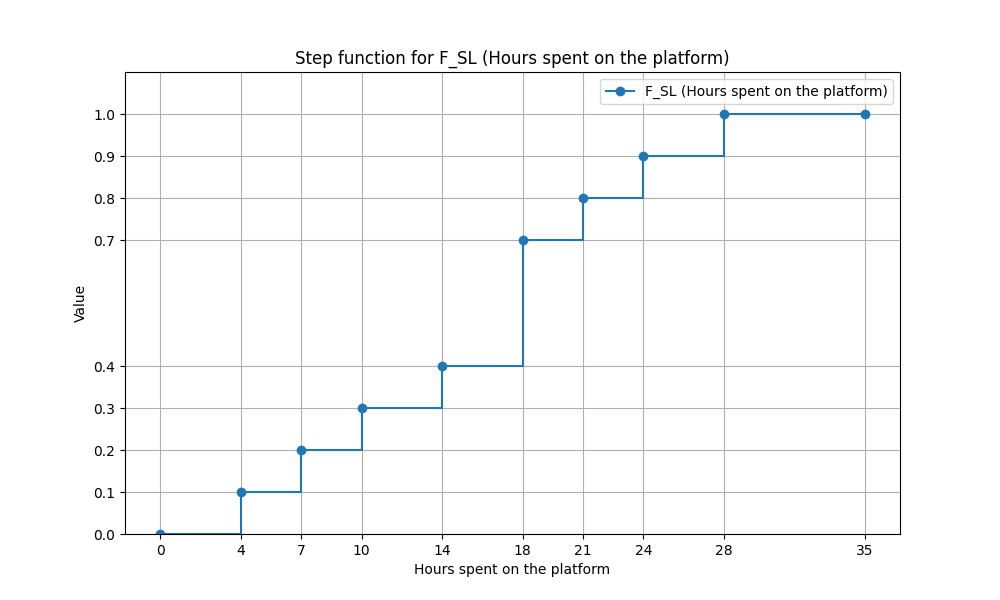
\includegraphics[width=\textwidth]{./assets/plot_F_SL.png}
    \caption{F\_SL Membership Function}
    \label{fig:plot_F_SL}
\end{figure}
This function is implemented this way because the company would prefer that users spend 28 hours per week on the platform. A higher number of hours is not rewarded further. At 18 hours there is a gap because the company wants to differentiate those who use the platform greatly from those who use it lightly.
\subsubsection{F\_FQ}
\begin{figure}[H]
    \centering
    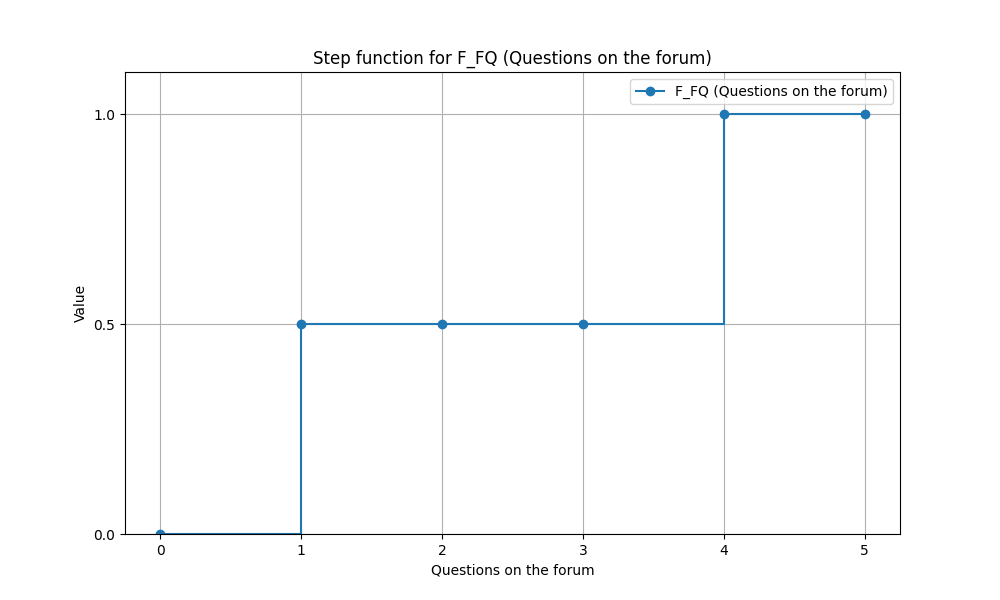
\includegraphics[width=\textwidth]{./assets/plot_F_FQ.png}
    \caption{F\_FQ Membership Function}
    \label{fig:plot_F_FQ}
\end{figure}
This function is implemented this way because the company wants to differentiate between those who do not ask questions, those who ask some questions, and those who ask many questions.
\subsubsection{F\_NA}
\begin{figure}[H]
    \centering
    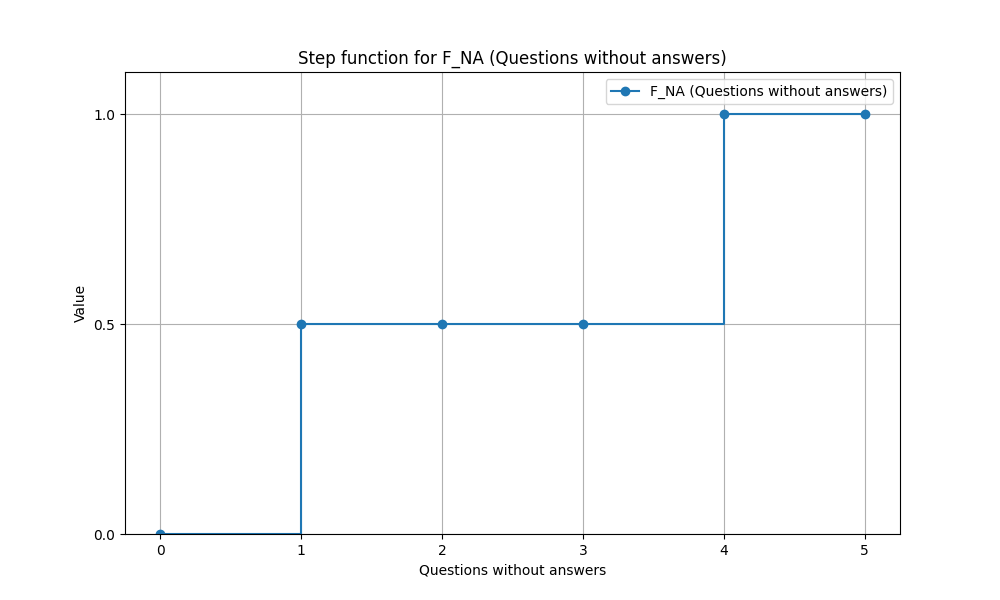
\includegraphics[width=\textwidth]{./assets/plot_F_NA.png}
    \caption{F\_NA Membership Function}
    \label{fig:plot_F_NA}
\end{figure}
This function is made this way because the company wants to understand whether users' questions catch the attention of others or not.
\subsubsection{F\_M}
\begin{figure}[H]
    \centering
    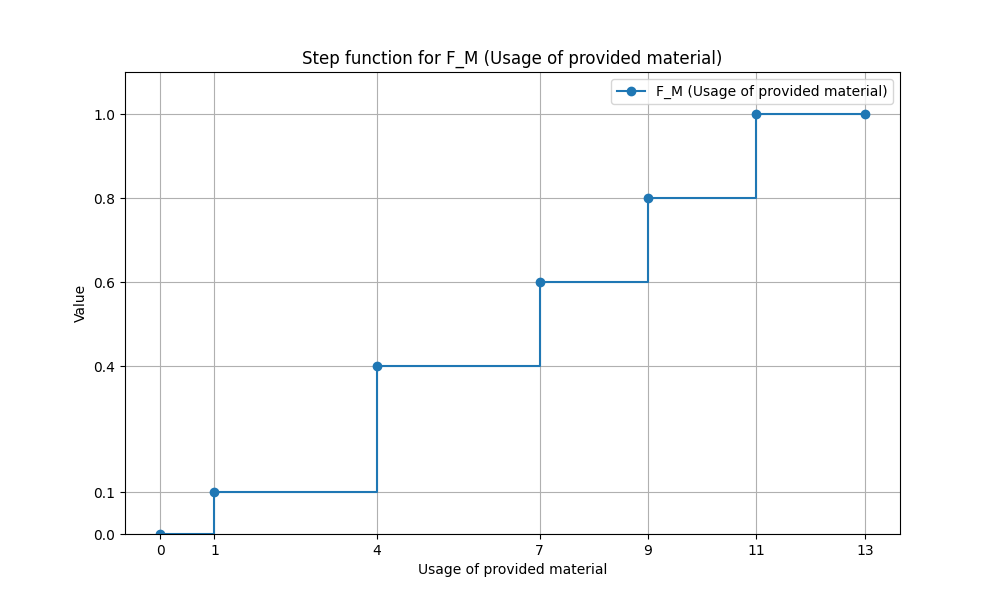
\includegraphics[width=\textwidth]{./assets/plot_F_M.png}
    \caption{F\_M Membership Function}
    \label{fig:plot_F_M}
\end{figure}
This function is implemented this way because the company wants the provided material to be partitioned equally over the entire duration of the training. The optimal amount is 11; using more is not rewarded further.

\subsection{Weights and situation calculation}
Each context attribute has an associated weight. F\_SL, F\_FQ and F\_M are considered positive factors, where F\_SL is considered to be the most important. F\_NA is considered a negative factor with low relevance. This decision was made on the assumption that unanswered questions did not pique the interest of other users probably because they were not relevant in the context in which they were asked. Viewing this factor as negative penalizes those who ask an excessive number of questions on the forum in order to try to increase their engagement.

\begin{table}[H]
    \begin{center}
    \begin{tabular}{ | m{7cm} | m{4cm}| m{4cm} | } 
      \hline
      \textbf{Attribute} & \textbf{Context attribute}  & \textbf{Weight}  \\ 
      \hline
      Session length & F\_SL & 0.56 \\ 
      \hline
      Questions on the forum & F\_FQ & 0.12 \\
      \hline
      Unanswered questions on the forum & F\_NA & -0.1 \\
      \hline
      Used material & F\_M & 0.32 \\
      \hline
    \end{tabular}
    \end{center}
    \caption{Context attributes table}
\end{table}

To calculate the situation a student is in, we use the following formula:
\[ 
S = \sum_{i=1}^3  w_i \cdot CA_i  
\]
Where:
\begin{itemize}
    \item $CA_i$ is one of the context attributes defined above
    \item $w_i$ is the relative weight
    \item i=0,1,2,3
\end{itemize}
Extended form formula:
\[
S = w_{SL} \cdot F\_SL + w_{FQ} \cdot F\_FQ + w_{NA} \cdot F\_NA + w_M \cdot F\_M
\]

\section{Simulation}
We simulated on two time intervals. The first data is taken after 7 days from when 
the users signed up in the platform (for simplicity, we will refer to this data as "week 1"), 
while the second taking was done after 12 days (for simplicity, we will say "week 2"). Six users 
are considered.\\
During week 1:
\begin{itemize}
    \item Aldo and Matteo do not stay much on the platform. They use about half of the planned 
    material and they decide that it is easier to ask many things on the forum.
    \item Maya and Matilde use very little material but they still ask some questions on the forum. 
    They know the platform is monitoring them so they decide to leave their devices on idle on the
     platform.
    \item Filippo and Marta are very interested on the topics they are studying and use the planned 
    material for the week. Hovewer, Filippo does not find the forum very useful while Marta the exact 
    opposite.
\end{itemize}

The results:\\
\vspace{1em}
\begin{table}[H]
\centering
\begin{tabular}{l l}
\toprule
Name     & Engagement Level \\
\midrule
Aldo     & Low \\
Filippo  & High \\
Marta    & High \\
Maya     & Medium \\
Matilde  & Low \\
Matteo   & Low \\
\bottomrule
\end{tabular}
\caption{Results for Test Case Week 1}
\end{table}
\vspace{1em}

During week 2:
\begin{itemize}
    \item Aldo wants to make up for his shortcomings. He spends more time on the platform and is very 
    interested in multimedia content.
    \item Filippo and Marta are still working very hard. Filippo has a personal commitment and spends 
    less time on the platform than in the previous week.
    \item Maya decides to stop cheating. She does not use the forum, spending all her time reading and 
    studying.
    \item Matilde wants to continue cheating. She thinks she needs to spend even more time online and 
    ask even more questions.
    \item Matthew continues his trend from the previous week. He completes more material, meanwhile,
    he interacts less on the forum. All his questions are answered.
\end{itemize}

The results:\\
\vspace{1em}
\begin{table}[H]
\centering
\begin{tabular}{l l}
\toprule
Name     & Engagement Level \\
\midrule
Aldo     & High \\
Filippo  & Medium \\
Marta    & High \\
Maya     & Medium \\
Matilde  & Medium \\
Matteo   & Medium \\
\bottomrule
\end{tabular}
\caption{Results for Test Case Week 2}
\end{table}
\vspace{1em}

These results show the achievement of our idea of engagement:
\begin{itemize}
    \item The most important element is the number of hours spent on the platform. You are able to 
    cheat by leaving devices on but with poor results without at least interacting with the forum.
    \item With a good number of hours and a good amount of material used engagement drops if there 
    is no interaction with the forum (unless the other parameters are perfect).
    \item The system is adaptive. The result can be recovered if user performance improves and, 
    also inversely, it drops as performance worsens.
\end{itemize}

\section{Dashboard Integration}
The CST is integrated into the dashboard through the script \textit{elasticsearch\_read\_injection.py}. 
This script creates a connection with Elastic Search, takes data from the 
\textit{users\_context\_attributes} index present inside Elastic Search (i.e., the data corresponding 
to week 1 of the simulation) and, for each user in the index, computes the corresponding engagement level, 
which is used to update the badge in the main dashboard. The values are then injected into Elastic Search 
in the \textit{users\_engagement\_level} index.